\section{Adaptive Memory Evolution}\label{sec:method}
\subsection{Causal flow and event updates}
At event $j$, the previous event's coefficients and context first evolve existing states through $\Delta_j=t_j-t_{j-1}$. Only then is the new event consumed. Let $q_i\in[0,1]$ denote held demand affinity and $v_i\in\{0,1\}$ indicate whether record $i$ is the latest \emph{observed} version of its addressed fact. Between events,
\begin{align}
\dot I_i&=\alpha_I k(0.5+wq_i-I_i), &
\dot C_i&=4\alpha_C k(v_i-C_i),\label{eq:flow}\\
\dot U_i&=-\alpha_U kU_i/20, & \dot T_i&=1.\nonumber
\end{align}
Importance $I_i$ relaxes toward current demand; consistency $C_i$ relaxes toward observed version status. Neither is an oracle of future utility or calibrated confidence. Usage $U_i$ decays to reduce inertia from past successful use. Temporal state $T_i$ ages between resets. For fixed held inputs, the update is exact:
\begin{equation}\label{eq:closed}
I_i'=b_i+(I_i-b_i)e^{-\alpha_I k\Delta},\quad
C_i'=v_i+(C_i-v_i)e^{-4\alpha_C k\Delta},\quad
U_i'=U_ie^{-\alpha_U k\Delta/20},\quad T_i'=T_i+\Delta,
\end{equation}
where $b_i=0.5+wq_i$. Zero strength skips its corresponding flow exactly. It does not disable observation/feedback jumps or the temporal clock.

The coefficient head maps a 32-dimensional content projection and eight causal features to three outputs $r\in\R^3$: insertion gate $g=\sigma(r_1)$, importance amplitude $w=2\sigma(r_2)$, and $k=(\operatorname{softplus}(r_3)+10^{-4})/30$. This affine head has 123 parameters, pretrained in a separate earlier development stage and frozen for every reported validation batch (Appendix~\ref{app:head}). There is no new optimization for rate sweeps. The rule control fixes $g=2/3,w=1.5,k=0.3$.

A newly observed version receives $(I,C,U,T)=(gw,1,0,0)$; shared bootstrap records have $I=1$. Reobserving a resident version applies $I\leftarrow\min(I+gw,20)$, $C\leftarrow1$, and $T\leftarrow0$. After retrieval, delivered feedback $y\in[0,1]$ updates the retrieved record by
\begin{equation}
C\leftarrow0.8C+0.2y,\qquad U\leftarrow U+y,\qquad T\leftarrow0.
\end{equation}
Absent records receive no update. Thus the system is hybrid: both elapsed time and discrete evidence matter.

\subsection{Retention, addressing, and interpretation}
An arriving candidate is temporarily added to the resident set. If this causes overflow, the lowest-scoring candidate or resident is removed, using
\begin{equation}\label{eq:score}
S_i=\log\max(I_i,10^{-8})+\log\max(C_i,0.05)+\log(1+U_i)-0.05\log(1+T_i).
\end{equation}
Away from the floors, this is $\log I_i+\log C_i+\log(1+U_i)-0.05\log(1+T_i)$. The floors are part of the implementation. Rejecting a write is distinct from evicting an existing resident. Version metadata can survive eviction, but evicted content cannot be retrieved. Structured retrieval chooses the newest resident version of the requested key; Equation~\ref{eq:score} controls availability, not answer ranking.

\begin{figure}[!htb]
\centering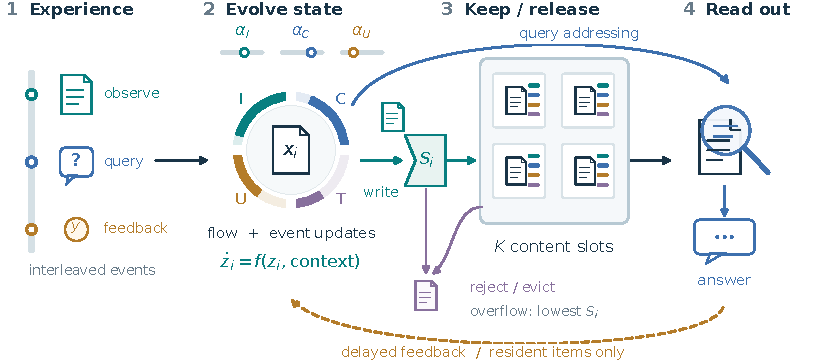
\includegraphics[width=\linewidth]{figures/framework.pdf}
\caption{Prior held inputs drive flow before each event; new inputs are held forward. Only overflowing writes trigger removal. Retrieval reads resident content, and feedback arrives later.}\label{fig:framework}
\end{figure}
The flow has a useful local guarantee: under held inputs, $I$ and $C$ remain between their starting states and targets, while $U$ contracts and $T$ increases. A proof and the assumptions needed to bound repeated usage increments appear in Appendix~\ref{app:properties}. This is a property of state evolution, not a guarantee of task accuracy: hard selection can switch discontinuously when score order changes.
